\documentclass[12pt]{article}

\usepackage[a4paper,margin=2cm,top=2cm,bottom=2cm,xetex]{geometry}
\usepackage[utf8]{inputenc}
\usepackage{color,xcolor}
\usepackage{graphicx,algorithm,algorithmic,booktabs,multirow, multicol,float,amsfonts}
\usepackage{enumitem}
\usepackage{amssymb}
\usepackage{amsthm}
\usepackage{amsfonts}
\usepackage{mathtools}
\usepackage{flexisym}
\usepackage{algorithm}
\usepackage{algorithmic}
\usepackage{tabularx}
\usepackage{listings}
\usepackage{xepersian}
\usepackage{amsmath}
\usepackage{physics}
\usepackage{colortbl}

\DeclareFixedFont{\ttb}{T1}{txtt}{bx}{n}{12} % for bold
\DeclareFixedFont{\ttm}{T1}{txtt}{m}{n}{12}  % for normal

% Custom colors
\usepackage{color}
\definecolor{deepblue}{rgb}{0,0,0.5}
\definecolor{deepred}{rgb}{0.6,0,0}
\definecolor{deepgreen}{rgb}{0,0.5,0}
\definecolor{lightred}{rgb}{1,0.8,0.8}
\definecolor{lightyellow}{rgb}{1,1,0.8}
\definecolor{lightblue}{rgb}{0.8,0.8,1}

\usepackage{listings}

% Python style for highlighting
\newcommand\pythonstyle{\lstset{
language=Python,
basicstyle=\ttm,
morekeywords={self},              % Add keywords here
keywordstyle=\ttb\color{deepblue},
emph={MyClass,__init__},          % Custom highlighting
emphstyle=\ttb\color{deepred},    % Custom highlighting style
stringstyle=\color{deepgreen},
frame=none,                         % Any extra options here
showstringspaces=false
}}


% Python environment
\lstnewenvironment{python}[1][]
{
\pythonstyle
\lstset{#1}
}
{}

% Python for external files
\newcommand\pythonexternal[2][]{{
\pythonstyle
\lstinputlisting[#1]{#2}}}

% Python for inline
\newcommand\pythoninline[1]{{\pythonstyle\lstinline!#1!}}

%\usepackage{mathtools}

\DeclareFontFamily{U}{matha}{\hyphenchar\font45}
\DeclareFontShape{U}{matha}{m}{n}{ <-6> matha5 <6-7> matha6 <7-8>
matha7 <8-9> matha8 <9-10> matha9 <10-12> matha10 <12-> matha12 }{}
%\DeclareSymbolFont{matha}{U}{matha}{m}{n}
%
%\DeclareMathSymbol{\nvartrianglelefteq}{\mathrel}{matha}{"9E}
%\DeclareMathSymbol{\vartrianglelefteq}{\mathrel}{matha}{"9C}

\newcount\HWcnt
\def\ttmp#1#2#3#4#5#6#7#8#9|{\def\Wjob{#9}}%
\expandafter\ttmp\jobname |
\def\ttmp#1#2#3{\global\HWcnt=#2#3}
\expandafter\ttmp\Wjob

\settextfont[Scale = 1.0 ,
             BoldFont = *Bd ,
             ItalicFont = *It ,
             BoldItalicFont = *BdIt ,
             Extension = .ttf
            ]{XB Niloofar}
\ExplSyntaxOn
\cs_set_eq:NN
\etex_iffontchar:D
\tex_iffontchar:D
\cs_undefine:N \c_one
\int_const:Nn \c_one { 1 }
\ExplSyntaxOff
\setdigitfont[Scale = 1.0 ,
             BoldFont = *Bd ,
             ItalicFont = *It ,
             BoldItalicFont = *BdIt ,
             Extension = .ttf
            ]{XB Niloofar}
\renewcommand{\baselinestretch}{1.2}
\pagestyle{empty}

\makeatletter
\def\abj@num@i#1{%
	\ifcase #1\or الف\or ب\or ج\or د\or ه\or و\or ز\or ح\or ط\fi \ifnum #1=\z@ \abjad@zero \fi
}
\renewcommand{\theenumi}{\abjad{enumi}}
\renewcommand{\labelenumi}{\theenumi)}
\long\def\makeHead#1{%
	\begin{center}\large
		\begin{tabular}{@{}p{.33\linewidth}<{\hfill}@{}>{\hfil}p{.33\textwidth}<{}@{}>{\hfill}p{.33\textwidth}@{}}
            \textbf{پاییز ۱۴۰۲} & & \textbf{تمرین ۱} \\[.5ex]
            \textbf{دکتر ریواده} & &  \textbf{ زمان آپلود: #1}\\[.5ex] 
            \hline\hline
		\end{tabular}
	\end{center}\smallskip
}

\newcommand{\Rule}{\ \hfill\rule{\linewidth}{0.5pt}\hfill\ \par\vspace*{-2ex}\par}
\newcommand{\DescRule}{\ \hfill\rule{\linewidth}{1pt}\hfill\ \vspace*{-2ex}\par}
\def\rank{\mathop{\mathrm{rank}}\nolimits}

\begin{document}
\makeHead{۱۸ آذر}
\begin{description}
%	\item{} \input{description.tex}
%	\DescRule

	\vspace*{-1cm}

	\item{\textbf{}} \section*{نام اعضای تیم و شماره دانشجویی‌ها}

سید ابوالحسن رضوی (402212655)

ایمان محمدی (99102207)

علی اسلامی نژاد (402211789)

شماره گروه: 20
	
	\newpage
	
	\vspace*{-2cm}
	
	\item{\textbf{}} \section*{جواب سوال ۱}

برای این سوال، طراحی در فیگما صورت گرفته است. لطفا به \href{https://www.figma.com/file/j9DWRQmEEL1pcwmt5AWs4E/HW3?type=design&node-id=0%3A1&mode=design&t=lIFq8iezIYotDbWQ-1}
{این لینک} مراجعه کنید.


\begin{figure}[H]
	\centering
	
\includegraphics{Frame 1.png}
	
	\label{fig:label4}
\end{figure}

\newpage

\begin{figure}[H]
	\centering
	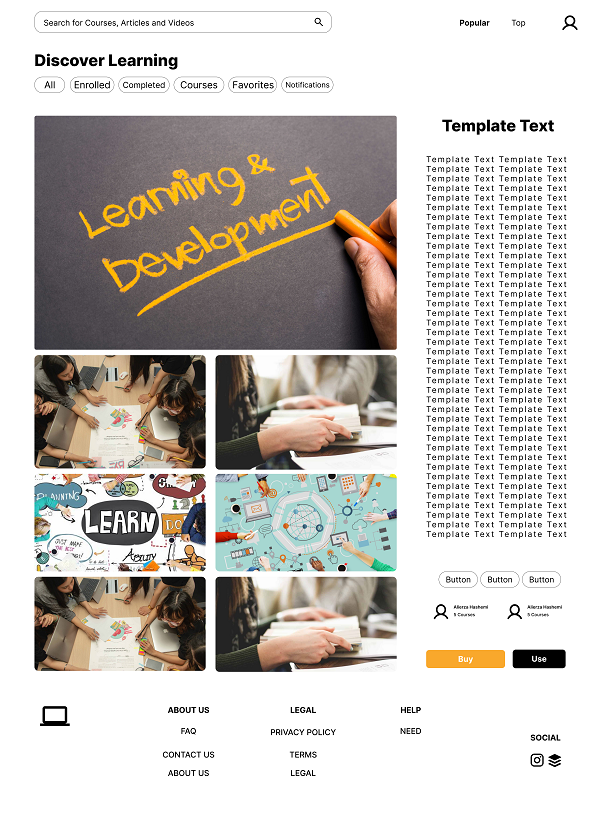
\includegraphics{Frame 2.png}
	
	\label{fig:label4}
\end{figure}
	
	\newpage
	
	\vspace*{-2cm}
	
	\item{\textbf{}} \section*{سوال ۲}

تفاوت فعالیت های تحلیل و طراحی سیستم های نرم‌افزاری را توضیح دهید. اطمینان حاصل کنید که در توضیحات خود به موارد زیر بپردازید:

\begin{itemize}
	\item ارتباط آن دو با یک مساله و راه حل آن
	\item اهداف و تمرکز هر یک
	\item سطح انتزاع هر کدام
	\item تقدم و تاخر هر یک از این دو فعالیت
	\item تفاوت مدل‌سازی ذیل هر فعالیت
\end{itemize}

\section*{جواب سوال ۲}

\subsection*{ارتباط با مساله و راه حل}
تحلیل نرم‌افزار به درک مسائل و نیازمندی‌های کاربران می‌پردازد و روی شناسایی و تعریف مشکلات تمرکز دارد. طراحی نرم‌افزار، از سوی دیگر، روی ارائه راه‌حل‌های فنی و ساختار سیستم برای برآورده ساختن این نیازمندی‌ها تمرکز دارد.

\subsection*{اهداف و تمرکز}
هدف از تحلیل نرم‌افزار شناسایی، جمع‌آوری و تعریف نیازمندی‌های کاربر است. در طراحی نرم‌افزار، تمرکز بر روی تعریف معماری، اجزا، رابط‌ها و دیگر جنبه‌های سیستم است.

\subsection*{سطح انتزاع}
تحلیل نرم‌افزار در سطح بالایی از انتزاع عمل می‌کند، به دنبال درک کلی مسائل و نیازمندی‌ها است. طراحی نرم‌افزار به سطح پایین‌تری از انتزاع می‌پردازد و به جزئیات فنی و ساختاری می‌پردازد.

\subsection*{تقدم و تاخر}
تحلیل نرم‌افزار معمولاً قبل از طراحی نرم‌افزار انجام می‌شود. تحلیل به شناسایی نیازمندی‌ها و مسائل می‌پردازد، در حالی که طراحی راه‌حل‌هایی برای این نیازمندی‌ها ارائه می‌دهد.

\subsection*{تفاوت در مدل‌سازی}
مدل‌سازی در تحلیل نرم‌افزار بر روی نمایش نیازمندی‌ها و مسائل تمرکز دارد، مانند دیاگرام‌های حالت و مورد استفاده. در طراحی نرم‌افزار، مدل‌سازی به ساختار و روابط بین اجزای سیستم می‌پردازد، مانند دیاگرام‌های کلاس و توالی.


	
	\newpage
	
	\vspace*{-2cm}
	
	\item{\textbf{}} \section*{سوال ۲}

سناریویی را در نظر بگیرید که در آن کاربر در حال تعامل با یک برنامه موبایل جدید است که برای مدیریت امور مالی شخصی طراحی شده است. این برنامه به کاربران امکان میدهد هزینه‌ها را پیگیری کنند، بودجه را تنظیم کنند و گزارش‌های مالی را مشاهده کنند. با این حال، کاربران برخی از مشکلات را هنگام استفاده از برنامه گزارش کرده‌اند. بر اساس اصول طراحی
\lr{Bruce Tognazzini}
 ، مشخص کنید کدام اصل(ها) ممکن است در این سناریو نقض شده باشد و دلایل آن را بیان کنید.

مشکلات گزارش شده:
\begin{itemize}
	\item برنامه اقدامات مربوطه را پیشنهاد نمی‌کند یا مراحل بعدی کاربر را پیش بینی نمی‌کند، مانند پیشنهاد تنظیم بودجه بر اساس الگوهای هزینه‌های گذشته.
	\item رابط برنامه با عملکردهای بیش از حد در صفحه اصلی به هم ریخته است، که تمرکز روی یک کار واحد مانند وارد کردن هزینه‌های روزانه را دشوار می‌کند.
	\item همینطور کاربران جدید گزارش کرده‌اند که درک نحوه پیمایش در برنامه و استفاده از ویژگی‌های آن مشکل دارند.
	\item ساختار \lr{Navigation} گیج‌کننده است بطوریکه برخی از عملکردها که در زیر چندین لایه از منوها مدفون شده‌اند و یافتن آنها را سخت می‌کند.
\end{itemize}

\section*{جواب سوال ۲}

بر اساس اصول طراحی \lr{Bruce Tognazzini}، چندین اصل ممکن است در این سناریو نقض شده باشند:

\begin{enumerate}
	\item \textbf{قابلیت پیش‌بینی \lr{(Predictability)}}: برنامه باید توانایی پیش‌بینی نیازهای کاربر و ارائه پیشنهادات مفید را داشته باشد. نبود این ویژگی در برنامه نشان‌دهنده نقض این اصل است. برای مثال، عدم پیشنهاد تنظیم بودجه بر اساس الگوهای هزینه‌های گذشته می‌تواند به ناکارآمدی در استفاده از برنامه منجر شود.
	
	\item \textbf{سادگی رابط کاربری \lr{(Simplicity)}}: رابط کاربری باید ساده و قابل فهم باشد. ازدحام عملکردها در صفحه اصلی موجب پیچیدگی و دشواری در استفاده می‌شود که نقض این اصل محسوب می‌شود. یک رابط کاربری بیش از حد پیچیده می‌تواند کاربران را سردرگم کند و تجربه کاربری را کاهش دهد.
	
	\item \textbf{قابلیت پیمایش \lr{(Navigability)}}: کاربران باید بتوانند به راحتی در برنامه حرکت کنند و به ویژگی‌های مختلف دسترسی داشته باشند. گیج‌کننده بودن ساختار 
	\lr{Navigation}
	نشان‌دهنده نقض این اصل است. وقتی کاربران نمی‌توانند به آسانی وظایف مورد نظر خود را در برنامه پیدا کنند، احتمال اینکه از استفاده از برنامه دست بکشند، افزایش می‌یابد.
	
	\item \textbf{وضوح و شفافیت \lr{(Clarity)}}: کاربران باید به راحتی بتوانند از عملکرد و نحوه استفاده هر قسمت از برنامه آگاه شوند. نبود شفافیت در نحوه پیمایش و استفاده از ویژگی‌ها، همچون مواردی که در ساختار Navigation یا عملکردهای پنهان در منوها مشاهده می‌شود، نشان‌دهنده نقض این اصل است.
	
	\item \textbf{پاسخگویی \lr{(Responsiveness)}}: برنامه باید به نیازهای کاربران به شکلی سریع و مؤثر پاسخ دهد. در صورتی که برنامه نتواند به سرعت و به طور مناسب به ورودی‌ها و درخواست‌های کاربران پاسخ دهد، این اصل نقض شده است.
\end{enumerate}
	
	\newpage
	
	\vspace*{-2cm}
	
	\item{\textbf{}} \section*{سوال ۳}

چرا ممکن است یک سیستم با عمر طولانی به اسناد طراحی بیشتری نیاز داشته باشد؟

\section*{جواب سوال ۳}

\section*{پشتیبانی و نگهداری}
اسناد طراحی کامل و به‌روز به تیم‌های مختلف کمک می‌کنند تا درک بهتری از سیستم داشته باشند، به ویژه در زمان انتقال مسئولیت نگهداری.

\section*{تغییرات و به‌روزرسانی‌ها}
اسناد طراحی دقیق می‌توانند به ثبت تغییرات و اطمینان از انسجام کلی سیستم در طول زمان کمک کنند.

\section*{کاهش خطای انسانی}
اسناد طراحی کامل به کاهش خطر از دست دادن دانش و تجربه مرتبط با سیستم و حفظ دانش حیاتی کمک می‌کنند.

\section*{سازگاری با محیط‌های جدید}
اسناد طراحی به شناسایی بخش‌هایی از سیستم که نیاز به تغییر یا به‌روزرسانی دارند، کمک می‌کنند، بویژه در زمان انطباق با فناوری‌های جدید.
	
	\newpage
	
	\vspace*{-2cm}
	
	\item{\textbf{}} \section*{سوال ۴}

\section*{\lr{.A}}
 چرا باید برای ایجاد یک نرم‌افزار براساس یک مدل پیش برویم و در طول پروژه پایبند به آن مدل باشیم؟

\section*{\lr{.B}}
یک تیم مهندس نرم‌افزار برای پروژه‌ای در یک شرکت نفت بزرگ دعوت شده است. این شرکت چندین دپارتمان دارد و تیم مهندسی نرم‌افزار با دپارتمان مدیریت اطلاعات (MIS) تعامل می‌کند. سیستم MIS این شرکت قدیمی (Legacy) است و هدف، انتقال داده‌ها به یک سیستم جدید (مهاجرت داده) است. فرآیندها، قراردادهای قانونی و معیارهای پذیرش این شرکت بسیار خاص و حساس هستند. به نظر شما چه مدل ایجاد نرم‌افزاری برای راه‌اندازی این سیستم انتقال داده را تیم مهندس نرم‌افزار انتخاب خواهد کرد؟ نام مدل و علت اصلی انتخاب آن کافی است.

\section*{\lr{.C}}
مهم‌ترین مشکلات مدل‌های سنتی (مثل مدل آبشاری) نسبت به مدل‌های چابک، چیست؟ ()اشاره به ۳ مورد و توضیح کامل آنها کفایت می‌کند.)

\section*{جواب سوال ۴}

\section*{\lr{.A} اهمیت استفاده از یک مدل در ایجاد نرم‌افزار}

\begin{itemize}
	\item \textbf{ساختار و راهنمایی:} مدل‌ها چارچوب و راهنمایی لازم را برای توسعه نرم‌افزار فراهم می‌کنند، کمک به تمرکز تیم بر اهداف و مراحل مشخص.
	\item \textbf{مدیریت پیچیدگی:} استفاده از یک مدل پیچیدگی‌ها را مدیریت می‌کند و اطمینان می‌دهد که تمام جنبه‌های پروژه پوشش داده شوند.
	\item \textbf{کنترل کیفیت:} پایبندی به مدل امکان بررسی و ارزیابی مرحله به مرحله پروژه را می‌دهد، که برای حفظ کیفیت نرم‌افزار ضروری است.
	\item \textbf{پیش‌بینی و برنامه‌ریزی:} مدل‌ها به تیم توسعه امکان پیش‌بینی و برنامه‌ریزی مناسب پیشرفت پروژه را می‌دهند.
	\item \textbf{همکاری و ارتباطات:} مدل‌ها زبان مشترکی برای ارتباط بین اعضای تیم و ذینفعان فراهم می‌کنند.
	\item \textbf{مستندسازی و توسعه مجدد:} مدل‌ها به مستندسازی فرایندها و تصمیمات کمک کرده و برای تحلیل و توسعه مجدد نرم‌افزار در آینده مهم هستند.
\end{itemize}

\section*{\lr{.B} مدل ایجاد نرم‌افزار برای شرکت نفتی}
\textbf{مدل انتخابی:}
مدل ترکیبی
\lr{(Hybrid Model)}
که ترکیبی از مدل آبشاری و چابک است.

\textbf{دلیل انتخاب:}

\begin{itemize}
	\item \textbf{پیچیدگی و حساسیت بالا:}
	 با توجه به پیچیدگی و حساسیت‌های موجود در فرآیندها و داده‌های شرکت نفتی، مدل ترکیبی اجازه می‌دهد تا بخش‌های حساس و پیچیده با دقت بالا و با رویکرد آبشاری پیاده‌سازی شوند.
	\item \textbf{انعطاف‌پذیری:}
	در بخش‌های کمتر حساس، استفاده از رویکردهای چابک به تیم اجازه می‌دهد تا به سرعت به تغییرات پاسخ دهد.
\end{itemize}

\section*{\lr{.C} مشکلات مدل‌های سنتی (مانند مدل آبشاری) نسبت به مدل‌های چابک}
\begin{itemize}
	\item \textbf{انعطاف‌پذیری کم:}
	مدل‌های سنتی اغلب انعطاف‌پذیری کمتری در برابر تغییرات دارند و تغییرات اساسی در مراحل پایانی پروژه دشوار است.
	\item \textbf{تأخیر در بازخورد:}
	در مدل‌های سنتی، بازخورد کاربران و ذینفعان معمولاً در مراحل پایانی پروژه جمع‌آوری می‌شود، که می‌تواند منجر به تأخیر در شناسایی و حل مشکلات شود.
	\item \textbf{ریسک بالا و هزینه‌های تغییر:}
	به دلیل تأخیر در دریافت بازخورد و انعطاف‌پذیری کم، ریسک شکست پروژه‌ها و هزینه‌های ایجاد تغییرات افزایش می‌یابد.
\end{itemize}
	
	\newpage
	
	\vspace*{-2cm}
	
	\item{\textbf{}} \section*{سوال ۶}

تفاوت «مدل ایجاد نرم‌افزار» مانند آبشاری یا حلزونی با «متدولوژی ایجاد نرم‌افزار» مانند XP یا RUP در چیست؟

انجمن علمی دانشکده مهندسی کامپیوتر خواستار «مدلی» برای برگزاری رویدادهای دانشجویی است. در طراحی این مدل، باید به ویژگی‌های زیر توجه شود:
\begin{itemize}
	\item حق‌الزحمه‌ای به نیروهای برگزارکننده پرداخت نمی‌شود.
	\item احتمال عدم انجام وظایف توسط برگزارکنندگان به دلیل عدم تعهد رسمی.
	\item دانشجویان وقت محدودی دارند.
	\item موضوعات رویداد حول مباحث رشته‌ی مهندسی کامپیوتر است.
	\item هدف اصلی، یادگیری و سپس لذت بردن از کار تیمی است.
	\item مخاطبین عمدتاً دانشجویان و دانش‌آموزان هستند.
\end{itemize}

\subsection*{موارد مورد توجه در طراحی}
\begin{itemize}
	\item جامعه مخاطبین
	\item ثبت‌نام مخاطبین
	\item جذب داوطلبین برگزاری
	\item انتخاب افراد داوطلب
	\item تخمین هزینه‌ها
	\item حامی مالی
	\item تبلیغات و برندینگ
	\item خط زمانی رویداد
	\item هماهنگی‌های اداری
\end{itemize}

با توجه به مدلی که در قسمت قبل تهیه کرده‌اید، متدولوژی‌ای برای برگزاری یک رویداد خاص طراحی کنید. این متدولوژی باید موقعیت خاصی را در نظر بگیرد و به صورت دقیق به ویژگی‌های آن بپردازد.

\textbf{توضیحات متدولوژی:} 
\begin{enumerate}
	\item تعریف موقعیت و ویژگی‌های رویداد
	\item تحلیل نیازمندی‌ها و محدودیت‌های رویداد
	\item برنامه‌ریزی جامع برای برگزاری
	\item پیاده‌سازی و اجرای رویداد
	\item ارزیابی و بازبینی پس از اتمام رویداد
\end{enumerate}

\section*{جواب سوال ۶}

تفاوت بین
\textbf{مدل ایجاد نرم‌افزار}
و
\textbf{متدولوژی ایجاد نرم‌افزار}
به نحوه‌ی دستورالعمل‌ها، فرآیندها، تکنیک‌ها و ابزارهایی برمی‌گردد که در هر کدام استفاده می‌شوند. بیایید این دو را با یکدیگر مقایسه کنیم:

\subsection*{مدل ایجاد نرم‌افزار:}

مدل ایجاد نرم‌افزار به الگوهای کلی مراحل و فعالیت‌های لازم برای توسعه نرم‌افزار اشاره دارد. این مدل‌ها معمولاً رویکردی سطح بالا به فرآیند توسعه نرم‌افزار دارند و می‌توانند مفاهیم مختلفی را در بر بگیرند که تیم‌ها باید دنبال کنند.

\begin{itemize}
	\item \textbf{آبشاری \lr{(Waterfall)} :}
یک مدل خطی و ترتیبی است که در آن هر مرحله باید کاملاً تمام شود قبل از اینکه مرحله بعدی شروع شود. مثال: ابتدا تحلیل نیازمندی‌ها، سپس طراحی سیستم، پس از آن پیاده‌سازی، تست و نهایتاً نگهداری.
	\item \textbf{حلزونی \lr{(Spiral)} :}
مدل حلزونی نیز مراحل آبشاری را دنبال می‌کند، اما با یک رویکرد تکراری که اجازه می‌دهد بازگشت به مراحل قبلی برای بهبود و اصلاح وجود داشته باشد. در هر دور، یک نسخه جدید و بهبود یافته از نرم‌افزار ساخته می‌شود.
\end{itemize}

\subsection*{متدولوژی ایجاد نرم‌افزار:}

متدولوژی ایجاد نرم‌افزار نه تنها مراحل کلی فرآیند توسعه را تعریف می‌کند، بلکه تکنیک‌ها، ابزارها، و دستورالعمل‌های دقیقی را برای هر مرحله ارائه می‌دهد. متدولوژی‌ها معمولاً بسیار جامع‌تر هستند و می‌توانند شامل توصیه‌هایی برای برنامه‌ریزی، تخمین زمان، مدیریت پروژه، توسعه و نگهداری باشند.

\begin{itemize}
	\item \textbf{\lr{XP (eXtreme Programming)} :}
یک متدولوژی چابک است که بر توسعه تکراری، برنامه‌ریزی مداوم، و بهبود مستمر تاکید دارد. همچنین، این متدولوژی بر توسعه به شیوه‌ی جفتی، تست محور و داشتن بازخورد مداوم از مشتری تأکید می‌کند.

	\item \textbf{\lr{RUP (Rational Unified Process)} :}
این متدولوژی یک فرآیند تکراری و افزایشی است که به تیم‌ها کمک می‌کند تا معماری نرم‌افزار را به خوبی تعریف کنند و مدیریت ریسک را در فرآیند توسعه ادغام کنند. RUP مجموعه‌ای از بهترین شیوه‌ها را در تمام جنبه‌های توسعه نرم‌افزار معرفی می‌کند.
\end{itemize}

بنابراین با توجه به تعریف‌هایی که داشتیم، تفاوت عمده در این است که مدل‌های توسعه نرم‌افزار بیشتر به الگوی کلی و توالی فعالیت‌ها توجه دارند، در حالی که متدولوژی‌های توسعه نرم‌افزار جزئیات دقیق‌تری از نحوه اجرای هر مرحله و اصول راهنما را ارائه می‌دهند و اغلب شامل راهنمایی‌های عملی‌تر و مشخص‌تر برای تیم‌های توسعه می‌شوند.

\begin{itemize}
	\item \textbf{تمرکز بر فرآیند:} مدل‌های ایجاد نرم‌افزار بیشتر روی فرآیند توسعه متمرکز هستند. آنها مراحل و توالی عمومی فعالیت‌های مورد نیاز برای تولید نرم‌افزار را تعریف می‌کنند.
	\item \textbf{جامعیت پایین‌تر:} مدل‌هایی مانند آبشاری یا حلزونی معمولاً دستورالعمل‌های مشخص و جزئی برای پیاده‌سازی فرآیندها ارائه نمی‌دهند. آن‌ها چارچوب‌های کلی هستند که نحوه به دنبال کردن هر مرحله را به تیم‌های توسعه واگذار می‌کنند.
	\item \textbf{انعطاف‌پذیری کمتر:} مدل‌ها مانند آبشاری سفت و سخت‌تر هستند و تغییرات را در میانه‌ی پروژه به خوبی تحمل نمی‌کنند.
	\item \textbf{پیش‌بینی‌پذیری:} این مدل‌ها به دلیل ترتیب مشخص شده‌شان پیش‌بینی‌پذیری بیشتری در مراحل توسعه فراهم می‌آورند، که می‌تواند برای مدیریت پروژه مفید باشد.
\end{itemize}

\subsection*{بررسی دقیق‌تر متدولوژی‌های ایجاد نرم‌افزار (مانند XP یا RUP ):}

\begin{itemize}
	\item \textbf{تمرکز بر جزئیات:} متدولوژی‌ها جزئیات دقیق‌تری از نحوه اجرای هر مرحله از فرآیند توسعه را فراهم می‌آورند، شامل روش‌ها، ابزارها، و دستورالعمل‌های خاص.
	\item \textbf{جامعیت بالاتر:} متدولوژی‌ها مجموعه‌ای از بهترین شیوه‌ها، قالب‌ها و استانداردهای صنعتی را ادغام می‌کنند که می‌تواند شامل توصیه‌های متعدد برای تمام جنبه‌های توسعه نرم‌افزار باشد.
	\item \textbf{انعطاف‌پذیری بیشتر:} متدولوژی‌ها مانند XP طراحی شده‌اند تا به تیم‌ها اجازه دهند به صورت چابک و با قابلیت پاسخگویی بالا به تغییرات پاسخ دهند.
	\item \textbf{تاکید بر بهبود مداوم:} متدولوژی‌ها اغلب شامل مکانیزم‌هایی برای بازنگری و بهبود مداوم فرآیندها هستند.
\end{itemize}

\subsubsection*{مثال:}

\begin{itemize}
	\item مدل آبشاری به شما می‌گوید که ابتدا نیازمندی‌ها را جمع‌آوری کنید، سپس طراحی کنید، پس از آن کدنویسی، سپس تست و در نهایت به تحویل محصول بپردازید. این یک توالی خطی و غیرقابل بازگشت است.
	\item متدولوژی RUP ، که یک متدولوژی تکراری و تدریجی است، به شما می‌گوید که چگونه باید نیازمندی‌ها را با استفاده از تکنیک‌های خاص جمع‌آوری کنید، چطور باید معماری را مدل‌سازی کنید، چگونه ریسک‌ها را مدیریت کنید و چطور فرآیندهای کدنویسی و تست را به صورت تکراری و با ادغام تغییرات انجام دهید.
\end{itemize}

\subsection*{ارائه‌ی مدل برای برگزاری رویدادهای انجمن علمی}

همان‌طور که می‌دانیم،
\lr{4MAT Learning Model}
مدلی برای طراحی تجربیات یادگیری و تدریس است که توسط دکتر برنیس مک‌کارتی توسعه یافته است. این مدل مبتنی بر این است که یادگیری در چهار فاز اصلی رخ می‌دهد: وابستگی (Why) ، تفکر (What) ، عملی (How) ، و ابداع (If) . با این حال، می‌توانیم از اصول این مدل برای طراحی و پیاده‌سازی مدل برگزاری رویدادهای دانشجویی استفاده کنیم. حالا در این مرحله، ما به تعریف دقیق هر مرحله از مدل خودمون می‌پردازیم و بررسی می‌کنیم که در هر مرحله چه کارهایی باید انجام شود و سپس تسک‌های تعریف شده در هر رویداد انجمن علمی را، اساین می‌کنیم به مراحل با توجه به تعاریفشان.

\subsubsection*{وابستگی (چرا؟ – Why ) :}

\textbf{هدف‌گذاری و انگیزه:}
در این مرحله، لازم است که انگیزه‌های برگزاری رویداد را مشخص کرده و به اعضا و داوطلبان بفهمانیم که چرا مشارکت آن‌ها اهمیت دارد. این کار با ارائه مزایای شرکت در رویدادها، مانند یادگیری و تجربه کار تیمی، انجام می‌شود. به‌خصوص باید در فرم جذب استف‌ها و صحبت‌های دبیر-نایب‌دبیر رویدادها با افراد خارج از رویداد، باید به مزایای شرکت در رویداد اشاره شود و همچنین برگزارکنندگان اصلی رویدادها باید تلاش کنند تا مزایای زیادی ایجاد کنند برای حضور در تیم برگزاری رویداد و تمرکزشان را روی یادگیری مهارت‌های نرم و سخت قرار دهند.

\subsubsection*{تفکر (چه چیزی؟ – What ) :}

\textbf{اطلاعات و داده‌ها:}
ارائه اطلاعات کلیدی در مورد رویداد، موضوعات، مخاطبین هدف، و فرآیند برگزاری به داوطلبان و شرکت‌کنندگان. این شامل توزیع دستورالعمل‌های دقیق، برنامه‌ها و مواد آموزشی است. در واقع، در این مرحله اطلاعات کلی و جزئی مربوط به نحوه‌ی شرکت در رویداد، نحوه‌ی استف شدن در رویداد، جزئیات شیوه‌ی برگزاری رویداد، مکان برگزاری‌ها، اطلاعات مربوط به شبکه‌های اجتماعی و باقی موارد، به اطلاع مخاطبان می‌رسد. این روند از طریق سوشال مدیاهای رویداد و همچنین کلامی می‌تواند شکل بگیرد.

\subsubsection*{عملی (چگونه؟ – How ) :}

\textbf{فرایند برگزاری:}
توسعه یک نقشه عملی برای برگزاری رویداد که شامل جذب داوطلبین، ثبت‌نام، تخمین هزینه‌ها، جذب حامی مالی، تبلیغات و برندینگ، خط زمانی رویداد و هماهنگی‌های اداری می‌شود. در این فاز باید دستورالعمل‌های عملی و واضحی برای هر یک از این بخش‌ها ارائه شود. این بخش خیلی دقیق به روند برگزاری رویداد می‌پردازد و نحوه‌ی برگزاری را مشخص می‌کند. در این‌جاست که دبیر-نایب‌دبیر رویدادها، درباره‌ی موارد مختلف مربوط به رویدادها تصمیم‌گیری می‌کنند و برنامه‌ی شیوه‌ی برگزاری را می‌ریزند. 

\subsubsection*{ابداع (اگر چه چیزی؟ – If ) :}

\textbf{بازخورد و بهبود:}
در این مرحله، فرصتی برای ارزیابی و بازاندیشی فراهم می‌شود. پس از هر رویداد، تیم برگزاری باید دور هم جمع شوند و در مورد آنچه خوب پیش رفت و چه چیزهایی نیاز به بهبود دارند بحث کنند. این مرحله همچنین فرصتی برای بررسی احتمالات جدید و نوآوری‌های احتمالی در رویدادهای آتی است.


	\hfill\textbf{}
\end{description}
\end{document}